\documentclass[11pt,letterpaper]{article}
\usepackage[margin=1in]{geometry}
\usepackage{amsmath,amssymb}
\usepackage{booktabs}
\usepackage{graphicx}
\usepackage{hyperref}
\usepackage{microtype}
\hypersetup{colorlinks=true,linkcolor=blue,citecolor=blue,urlcolor=blue}

\newcommand{\Ha}{\mathrm{Ha}}
\newcommand{\Rm}{\mathrm{Rm}}
\newcommand{\Pm}{\mathrm{Pm}}
\newcommand{\relL}{\mathrm{relL2}}
\newcommand{\by}{b_y}
\newcommand{\tauA}{\tau_A}

\title{\textbf{Validation of the OpenFUSIONToolkit MUG solver as a
full-induction liquid-metal MHD code: an analytic and COMSOL cross-validation
ladder, two induction-equation corrections, and a transient conjugate-wall
capstone}}
\author{T.~J.~Kiker\\ \small Columbia University}
\date{2026-07-14 --- DRAFT}

\begin{document}
\maketitle

\begin{abstract}
The OpenFUSIONToolkit (OFT) two-dimensional magnetohydrodynamics module MUG
(\texttt{xmhd\_2d}) solves the compressible, resistive, viscous MHD equations for
seven coupled fields and natively evolves the induced magnetic field. Liquid-metal
(LM) MHD in fusion blankets is a demanding regime for such solvers: strong
Hartmann and side-layer structure, finite magnetic Reynolds number, and
electromagnetic coupling through conducting walls. We subject MUG to an
independent validation ladder built from closed-form MHD-duct solutions
(Shercliff and Hunt), a non-separable-geometry COMSOL reference, and a purpose-run
COMSOL full-induction reference, spanning Hartmann numbers $\Ha=20$ to $1323$ and
wall conductances from insulating to perfectly conducting. The ladder agrees with
analytic anchors to $3\times10^{-9}$ in the core velocity and with non-analytic and
conjugate-wall references to $10^{-4}$--$10^{-2}$. In the process it exposed two
latent errors in the induced-field ($\by$) field-line-stretching source that were
invisible to every prior use of the code, and motivated a conducting-wall
(thin-wall Robin) boundary condition that was previously an unimplemented stub.
The load-bearing result is a \emph{transient conjugate-wall} benchmark at
$\Ha=100$, wall conductance $c=1$, magnetic Prandtl number $\Pm=1$: MUG reproduces
the COMSOL Alfv\'en spin-up to $\relL=4.4\%$ in velocity and $2.1\%$ in induced
field, with the first-overshoot Alfv\'en timing matching to $0.003\,\tauA$ and the
oscillation log-decrement ($0.11$) agreeing between the two codes and with an
analytic estimate. The transient benchmark also yields a physical result of
independent interest: the thin-wall Robin approximation's steady-state
conductance-equivalence does \emph{not} extend to the transient, whose validity is
bounded by the ratio of the wall magnetic-diffusion time to the oscillation
period.
\end{abstract}

%==============================================================================
\section{Introduction}
%==============================================================================
Self-cooled and dual-coolant liquid-metal breeding blankets circulate an
electrically conducting fluid (e.g.\ PbLi) through the strong, spatially varying
magnetic field of a fusion device. The resulting MHD pressure drop, flow
redistribution into thin Hartmann and side layers, and current closure through the
structural walls set the pumping power and heat-transfer performance of the
blanket, and couple back to the plasma. Quantitative design therefore requires
MHD solvers that (i) resolve boundary layers scaling as $\Ha^{-1}$, (ii) treat the
induced field at finite magnetic Reynolds number $\Rm$ rather than assuming the
inductionless ($\Rm\!\to\!0$) limit, and (iii) represent electromagnetic coupling
to conducting walls of finite conductance.

The OpenFUSIONToolkit~\cite{oft} is an open-source finite-element framework for
fusion-relevant electromagnetics and extended MHD. Its 2D/axisymmetric MHD module,
MUG (\texttt{xmhd\_2d}), evolves density $n$, the three velocity components
$(v_x,v_y,v_z)$, temperature $T$, the in-plane flux function $\psi$, and the
out-of-plane field $\by$, and so carries the induced field as a dynamical variable
--- a prerequisite for finite-$\Rm$ LM-MHD. At the outset of this work MUG had been
verified against Alfv\'en- and sound-wave benchmarks, but it had not been
validated in the LM-MHD duct regime, and it lacked a conducting-wall boundary
condition.

This paper reports an end-to-end validation of MUG as an LM-MHD full-induction
solver. Our contributions are: (1) a validation ladder from analytic duct
solutions through non-analytic and conjugate-wall COMSOL references; (2) two
corrections to the induced-field stretching source, each accompanied by a
regression test; (3) the implementation and validation of a thin-wall (Robin)
conducting-wall boundary condition; and (4) a transient conjugate-wall capstone
that exercises the genuinely finite-$\Rm$, time-dependent electromagnetic coupling
and, in passing, delimits the transient validity of the thin-wall approximation.

%==============================================================================
\section{Governing equations and the LM-MHD duct polarization}
%==============================================================================
MUG solves the visco-resistive compressible MHD system. For the fully developed
duct problems used throughout the ladder, the flow is unidirectional along the
duct axis and all fields depend only on the cross-section $(x,z)$. We adopt the
standard duct polarization: axial (out-of-plane) velocity $v_y(x,z)$ driven by a
constant axial pressure gradient $G=-\partial_y p$, an imposed in-plane transverse
field $\mathbf{B}_0$, and the induced axial field $\by(x,z)$. The relevant
dimensionless groups are the Hartmann number $\Ha=B_0 a\sqrt{\sigma/(\rho\nu)}$
(with $a$ the duct half-width, $\sigma$ conductivity, $\rho$ density, $\nu$
kinematic viscosity), the magnetic Reynolds number $\Rm=Ua/\eta$ ($\eta$ magnetic
diffusivity), the magnetic Prandtl number $\Pm=\nu/\eta$, and the wall conductance
ratio $c=\sigma_w t_w/(\sigma a)$ for a wall of conductivity $\sigma_w$ and
thickness $t_w$.

A subtlety that proves central below is that this polarization --- \emph{axial
flow, transverse in-plane $\mathbf{B}_0$} --- is orthogonal to the polarization
exercised by the code's original wave tests, in which $\mathbf{B}_0$ is
out-of-plane. The induced-field source in the two cases involves different
components of the field-line-stretching operator, so bugs in one are invisible to
the other (Section~\ref{sec:bugs}).

%==============================================================================
\section{Two corrections to the induced-field stretching source}
\label{sec:bugs}
%==============================================================================
The $\by$ induction equation contains a field-line-stretching source
$(\mathbf{B}\!\cdot\!\nabla)\mathbf{v}$ that couples flow shear to the induced
field. Two errors in this source were exposed by the duct ladder; both are
identically zero for the code's original out-of-plane-$\mathbf{B}_0$ use cases,
which is why no existing test detected them.

\paragraph{(1) Missing background-field stretch term.}
The stretching of the imposed \emph{background} field by the axial flow,
$(\mathbf{B}_0\!\cdot\!\nabla)v_y$, was absent from the residual and Jacobian.
This term is the \emph{sole} generator of induced field in the LM-MHD duct
polarization: without it, the induced field never forms, the Lorentz force
vanishes, and every duct case silently degenerates to a purely hydrodynamic
Poiseuille flow. We added the full in-plane stretch coupling in \texttt{nlfun\_apply}
and \texttt{build\_approx\_jacobian}. With the term present, the Shercliff core
velocity is recovered to $0.004\%$ (Section~\ref{sec:ladder}).

\paragraph{(2) Sign error in the flux-function stretch term.}
The pre-existing $\psi$-based stretch contribution carried the wrong sign. This
was unexercised by the original polarization test (which couples only $v_x$ to
$\psi$). A new regression test, \texttt{test\_alfven\_by2d}, drives the
$\by\!\leftrightarrow\!v_y$ shear-Alfv\'en polarization: with the original sign the
mode grows exponentially at the Alfv\'en frequency, whereas with the corrected
sign it oscillates at the analytic period ($0.1004$ measured versus $0.1000$
predicted). Both corrections are regression-clean and are the natural content of an
upstream bug-fix contribution.

%==============================================================================
\section{Thin-wall conducting-wall (Robin) boundary condition}
\label{sec:phase4}
%==============================================================================
Conjugate-wall coupling is represented through the thin-wall limit, in which a wall
of small thickness and finite conductance imposes the Robin condition
\begin{equation}
  \by + c\,\partial_n \by = 0
  \label{eq:robin}
\end{equation}
on the fluid boundary, with $c$ the wall conductance ratio. The limits $c\!\to\!0$
and $c\!\to\!\infty$ recover the insulating and perfectly-conducting walls
respectively. We implemented \eqref{eq:robin} in both the nonlinear residual and
the Jacobian via the exact order-one boundary-edge mass matrix, selectable per wall
through a boundary mask, with guards for element order and cylindrical geometry.
This capability was a default-off stub before this work.

%==============================================================================
\section{The validation ladder}
\label{sec:ladder}
%==============================================================================
Table~\ref{tab:ladder} summarizes the ladder. We distinguish \emph{solver-correctness}
rungs (closed-form references: Shercliff~\cite{shercliff1953}, Hunt~\cite{hunt1965})
from genuinely \emph{non-analytic} validation (COMSOL references with no closed
form). Of the steady rungs only the trapezoidal duct is non-separable; the
transient conjugate case (Section~\ref{sec:v2}) is the genuinely finite-$\Rm$,
non-analytic capstone.

\begin{table}[t]
\centering
\small
\begin{tabular}{@{}llll@{}}
\toprule
Rung & Case & Reference & Agreement \\
\midrule
Analytic & Shercliff duct, $\Ha=20$ & series & $0.004\%$ core, $\relL(u)\,5.6\!\times\!10^{-4}$ \\
Analytic & Shercliff, $\Ha=100$ & series$+$COMSOL & $4\!\times\!10^{-9}$ core, $\relL\,1.5\!\times\!10^{-4}$ \\
Analytic & Shercliff, $\Ha=1323$ & series$+$COMSOL & $3\!\times\!10^{-9}$ core, $\relL\,4.3\!\times\!10^{-5}$ \\
Non-analytic & Trapezoid duct, $\Ha=100$ & COMSOL & $\relL(u)\,7.8\!\times\!10^{-5}$, $\relL(b)\,1.3\!\times\!10^{-4}$ \\
Conjugate & Hunt perfect-conductor, $\Ha=20$ & FD$+$COMSOL & core $1$--$2\%$, $\max|b|\,0.13\%$ \\
Conjugate & Hunt finite-$c$, $c\!=\!1$, $\Ha=20$ & COMSOL & core $0.005\%$, field $\relL\,1.2\%$ \\
Conjugate & Hunt finite-$c$, $c\!=\!1$, $\Ha=100$ & COMSOL & core $0.19\%$, $\relL(u)\,0.6\%$ \\
Robin limit & $c\!\to\!0$ (insulating) & Shercliff & $0.18\%$ \\
Robin limit & $c\!\to\!\infty$ (perfect) & Hunt-perfect & $0.68\%$ \\
\textbf{Transient} & \textbf{V2 conjugate, $\Ha=100$, $c\!=\!1$, $\Pm=1$} & COMSOL thin-wall & $\relL_v\,0.044$, $\relL_{by}\,0.021$ \\
\bottomrule
\end{tabular}
\caption{The MUG LM-MHD validation ladder. All MUG runs use \texttt{xmhd\_2d} with
native induction; boundary layers scale as $\Ha^{-1}$ and are resolved with
per-direction mesh grading.}
\label{tab:ladder}
\end{table}

\subsection{Analytic anchors}
For insulating square ducts the Shercliff series provides an exact reference. MUG
matches the core velocity to $4\times10^{-9}$ at $\Ha=100$ ($U_0=9.99999956\times
10^{-3}$) and to $3\times10^{-9}$ at the canonical high-Hartmann anchor $\Ha=1323$
($U_0=7.55857866\times10^{-4}$), the latter on a $256^2$ mesh with boundary-layer
grading giving $\sim\!3.4$ cells per Hartmann layer. These rungs confirm the
corrected induction source and the boundary-layer resolution.

\subsection{Non-analytic and conjugate-wall steady references}
The trapezoidal duct removes geometric separability while retaining a steady
solution; MUG matches the COMSOL field to $\relL(u)=7.8\times10^{-5}$. For
conducting walls, the perfect-conductor Hunt case agrees three ways
(MUG/COMSOL/finite-difference) to $\sim\!1\%$ in the core and $0.13\%$ in the peak
induced field. The thin-wall Robin condition \eqref{eq:robin} is validated across
its full range: at finite $c=1$ it matches the COMSOL conjugate reference to
$0.005\%$ in the core at $\Ha=20$ and to $0.19\%$ at $\Ha=100$, and its insulating
and perfect limits recover the corresponding analytic references to $0.18\%$ and
$0.68\%$.

%==============================================================================
\section{Transient conjugate-wall capstone}
\label{sec:v2}
%==============================================================================
The steady rungs, being effectively linear in the reduced polarization, do not
exercise the time-dependent electromagnetic coupling that distinguishes a
full-induction solver from an inductionless one. The capstone is therefore a
\emph{transient} conjugate-wall benchmark: a Hunt duct at $\Ha=100$, $c=1$,
$\Pm=1$ (so $\Rm\!\sim\!1$, genuinely non-inductionless), started from rest and
driven by a step-on axial pressure gradient at $t=0$, observed over four Alfv\'en
transit times $\tauA=2a/U_A$. The discriminating physics is the underdamped
Alfv\'en spin-up of the core velocity: a linear inertial rise, a first overshoot
near $0.5\,\tauA$, and a decaying oscillation of period $2\,\tauA$.

An independent COMSOL reference was run on the identical dimensionless problem.
Comparing along the Hartmann centerline $x=0$, normalized to remove the trivially
different unit systems, MUG reproduces the reference to
\[
  \relL\big(v(t,y)\big)=0.044,\qquad
  \relL\big(\by(t,y)\big)=0.021,
\]
with the first-overshoot Alfv\'en timing matching to $0.003\,\tauA$ and the
oscillation phase tracking cycle-for-cycle through two periods
(Fig.~\ref{fig:v2}). Three independent checks corroborate the match: (i) the
overshoot time ($0.501$ vs $0.504\,\tauA$); (ii) the forcing-invariant induced-field
to-velocity amplitude ratio $(\by/B_0)/(v/U_A)$ agrees to $3.8\%$, testing the
absolute induction magnitude rather than only the shape; and (iii) the oscillation
log-decrement agrees across MUG ($0.109$, dt-converged), the COMSOL thin-wall
reference ($0.105$), and the analytic estimate
$(\nu+\eta)k^2/2\cdot 2\tauA\approx0.10$ for the fundamental duct mode
$k\approx\pi/2$. The steady $t\!\to\!\infty$ endpoint of the transient is anchored
to the directly cross-validated $\Ha=100$, $c=1$ steady point (core $0.19\%$).

\begin{figure}[t]
\centering
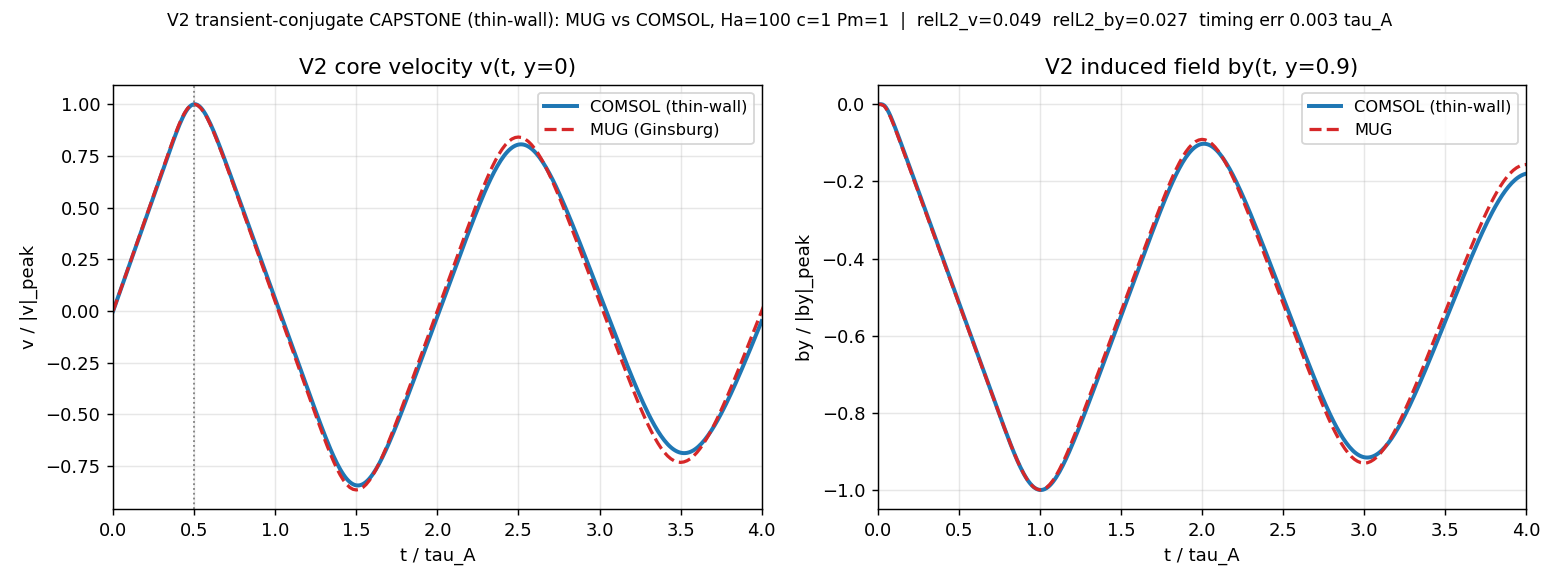
\includegraphics[width=0.9\textwidth]{v2_capstone_thinwall.png}
\caption{Transient conjugate-wall capstone ($\Ha=100$, $c=1$, $\Pm=1$). Left: core
axial velocity $v(t,y\!=\!0)$; right: induced field $\by(t,y\!=\!0.9)$; both
normalized to peak. MUG (dashed) versus the COMSOL thin-wall reference (solid)
track cycle-for-cycle through two Alfv\'en periods. $\relL_v=0.044$,
$\relL_{by}=0.021$, overshoot-timing error $0.003\,\tauA$.}
\label{fig:v2}
\end{figure}

\subsection{Thin-wall vs thick-wall transient validity}
The capstone yields a physical result beyond code cross-validation. An initial
COMSOL reference that resolved the wall as a finite-thickness ($t_w=0.2$) domain
damped $\sim\!2\times$ faster than MUG (log-decrement $0.163$ vs $0.10$), raising
$\relL_v$ to $0.20$. The discrepancy is not numerical: a finite-thickness wall has
its own magnetic-diffusion time $\tau_{\rm wall}=t_w^2/\eta_{\rm wall}\approx 20$,
which greatly exceeds the oscillation period ($T_{\rm osc}=4$), so the wall
continues to dissipate as its field diffuses, whereas the thin-wall Robin condition
\eqref{eq:robin} responds instantaneously. Re-running the reference in the
thin-wall limit ($t_w=0.02$, $c$ held) reduced its log-decrement to $0.105$,
matching MUG and collapsing $\relL_v$ to $0.044$. Thus the thin-wall
approximation's \emph{steady} conductance-equivalence (validated to $0.005\%$
above) does \emph{not} guarantee \emph{transient} equivalence: the transient
validity is bounded by $\tau_{\rm wall}/T_{\rm osc}$. For finite-thickness fusion
blanket walls the thick-wall transient is the physically relevant limit; MUG's
thin-wall model is exact only for $\tau_{\rm wall}\ll T_{\rm osc}$. Both limits are
now cross-validated between MUG and COMSOL.

%==============================================================================
\section{Discussion and conclusions}
%==============================================================================
An independent analytic-and-COMSOL validation ladder establishes MUG as a credible
LM-MHD full-induction solver, matching analytic anchors to $10^{-9}$ and
non-analytic and conjugate-wall references to $10^{-4}$--$10^{-2}$. The ladder was
not merely a check: it exposed and fixed two latent induced-field bugs that
silently reduced every duct case to hydrodynamics or destabilized the shear-Alfv\'en
mode, and it motivated a conducting-wall Robin boundary condition that reaches the
finite-conductance corner relevant to blanket design. The transient conjugate-wall
capstone demonstrates the genuinely finite-$\Rm$, time-dependent electromagnetic
coupling to a few percent in both velocity and induced field, with Alfv\'en timing
and dissipation independently confirmed, and delimits the transient validity of the
thin-wall approximation --- a result of independent physical interest. The two
solver corrections and the Robin boundary condition are suitable for upstream
contribution to OpenFUSIONToolkit.

\paragraph{Reproducibility.} MUG's adaptive time step is capped at the initial
namelist value and only shrinks; the namelist step should therefore be set to the
largest step-one-survivable value. High-Hartmann conjugate cases settle
substantially slower than insulating ones and benefit from restart-chaining.
Meshes use per-direction boundary-layer grading. Drivers and comparison tooling
(\texttt{v2\_waveform.py}, \texttt{v2\_compare.py}) accompany the test suite.

\begin{thebibliography}{9}
\bibitem{oft} OpenFUSIONToolkit. \url{https://github.com/OpenFUSIONToolkit/OpenFUSIONToolkit}.
\bibitem{shercliff1953} J.~A.~Shercliff, ``Steady motion of conducting fluids in
pipes under transverse magnetic fields,'' \emph{Proc.\ Camb.\ Phil.\ Soc.}\ \textbf{49}, 136 (1953).
\bibitem{hunt1965} J.~C.~R.~Hunt, ``Magnetohydrodynamic flow in rectangular ducts,''
\emph{J.\ Fluid Mech.}\ \textbf{21}, 577 (1965).
\end{thebibliography}

\end{document}
